% !TEX root = graph2.tex

\documentclass[twocolumn]{article}
\usepackage{graphicx} % Required for inserting images
\usepackage{CJKutf8}
% \usepackage{amsthm}
\usepackage{mdframed}
\usepackage{multicol} % 用於分欄
\usepackage{geometry} % 用於調整頁面尺寸和邊距
\usepackage{amsmath}
\usepackage{titlesec}
\usepackage{float}
\usepackage{titlesec}


\titleformat{\section}{\small\bfseries}{\thesection}{1em}{}

\newtheorem{example}{example}             % 整体编号
\newtheorem{algorithm}{algorithm}
\newtheorem{theorem}{theorem}[section]  % 按 section 编号
\newtheorem{definition}{definition}
\newtheorem{axiom}{axiom}
\newtheorem{property}{property}
\newtheorem{proposition}{proposition}
\newtheorem{lemma}{lemma}
\newtheorem{corollary}{corollary}
\newtheorem{remark}{remark}
\newtheorem{condition}{condition}
\newtheorem{conclusion}{conclusion}
\newtheorem{assumption}{assumption}
\newtheorem{formula}{formula}
\newtheorem{problem}{problem}
\newtheorem{solution}{solution}
\newtheorem{fact}{fact}
\newtheorem{hw}{hw}

\linespread{0.1}
% \setlength{\parskip}{0.001em}

\setlength{\topsep}{0.01em} % 環境之上和之下的距離
\setlength{\partopsep}{0pt} % 環境和上下文之間的額外距離
\setlength{\itemsep}{0.5em} % 項目之間的距離
\setlength{\parsep}{0pt} % 段落之間的距離

\titlespacing*{\section}{0pt}{0pt}{0pt}

% 設定頁面尺寸和邊距
\geometry{
    top=0.1cm,
    bottom=0.1cm,
    left=0.1cm,
    right=0.1cm
}


% 自定義 "Definition" 環境
% \newmdtheoremenv{definition}{Definition}
% \theoremstyle{mystyle}

\title{}
% \author{}
% \date{}

\begin{document}
\begin{CJK*}{UTF8}{bkai}

% \maketitle

% 第一部分(Chapter 1)
\section{matching}
    \begin{theorem}
     (Tutte 1947). A graph G has a 1-factor $\iff$ 
     o(G-S) $\leq$ |S| for every S $\subseteq $ V(G).
    \end{theorem}
% \vspace{2cm} % 分隔不同章節

    \begin{corollary}
       (Peterson 1891) Every 3-regular graph with no cut-edge has a 1-factor.  
    \end{corollary}

    \begin{definition}
        $defect_{G} = \max _{S \subseteq V(G)} o(G-S)-|S|$
    \end{definition}

    \begin{theorem}
        (Berge-Tutte Formula, Berge 1958). The maximum number of vertices saturated by a matching in G is
 n(G) -defectG = min
 $S \subseteq V(G)$
 (n(G) -(o(G-S)-|S|))
    \end{theorem}

% 第二部分(Chapter 2)
\section{Connectivity}
% \begin{multicol}{2} % 第二部分分欄
    % \switchcolumn[0]

    \begin{definition}{}
         A separating set or vertex cut of a graph G is a set S ⊆ V(G) s.t. G−S has
 more than one component.
    \end{definition}

    \begin{definition}
         The connectivity of G, written $\kappa$(G), is the minimum size of a vertex set S s.t.
 G-S is disconnected or has only one vertex. A graph G is k-connected if
 $\kappa$(G) $\geq$ k, i.e., G-S is connected with at least two vertices for every
 k -1-vertex set S.
    \end{definition}

    \begin{lemma}
        $\kappa$(G) = n(G)-1 $\iff$ G contains Kn(G), i.e., every vertex is adjacent to every
 other vertex.
    \end{lemma}

    \begin{definition}
         A disconnecting set of edges is a set F $\subseteq $ E(G) s.t. G-F has more than one
 component.
    \end{definition}

    \begin{definition}
         A graph is k-edge-connected if every disconnecting set has at least k edges.
 The edge-connectivity of G, written $
 \kappa$'(G), is the minimum size of a
 disconnecting set or equivalently, the maximum k s.t. G is k-edge-connected
    \end{definition}

    \begin{fact}
    Every edge cut is a disconnecting set.
    \end{fact}

    \begin{fact}
         Every minimal disconnecting set of edges is an edge cut.
    \end{fact}

    \begin{definition}
        $\delta (G)$ = minimum vertex degree of G
    \end{definition}

    \begin{theorem}{ (Whitney 1932).}
         $\kappa (G) \leq \kappa '(G) \leq \delta (G)$ for every graph G.
    \end{theorem}

    \begin{theorem}
         If G is a 3-regular graph of order more than 2, then $\
         kappa $(G) = $\kappa $'(G).
    \end{theorem}

    \begin{definition}
         Two paths are internally disjoint if they do not have common internal vertices.
         Two x,y-paths are edge-disjoint if they do not share any edges
        \end{definition}

    \begin{theorem}{(Whitney)}
         A graph G having at least 3 vertices is 2-connected $\iff$ for every distinct
 u,v $\in$ V(G) there exist internally disjoint u,v-paths in G.
    \end{theorem}

    \begin{lemma}{(Expansion Lemma)}
        If G is k-connected, and G' is obtained from G by adding a new vertex y with
 at least k neighbors in G, then G' is k-connected.
    \end{lemma}

    \begin{theorem}
         For a graph G of order at least 3, the following conditions are equivalent and
 characterize 2-connected graphs.

 \begin{itemize}
    \item G is connected and has no cut-vertex.
 \item For all x,y $\in$ V(G) there are internally disjoint x,y-paths.
 \item For all x,y $\in$ V(G) there is a cycle through x and y.
 \item $\delta$(G) $\geq$ 1 and every pair of edges in G lies on a common cycle.\end{itemize}
    \end{theorem}

    \begin{definition}
         A subdivision of an edge e = xy is a replacement of e with path x,z,y where z
 is a new vertex.
    \end{definition}

    \begin{corollary}
         If G is 2-connected, then the graph G' obtained by subdivision of an edge
 e =xy of G is 2-connected.
    \end{corollary}

    \begin{definition}
         An ear of a graph G is a nontrivial path in G whose endpoints have degree at
 least 3 and all its internal vertices have degree 2.
    \end{definition}

    \begin{definition}
         A decomposition of a graph is a list of subgraphs s.t. every edge appears in
 exactly one subgraph in the list.
    \end{definition}

    \begin{definition}
         An ear decomposition of G is a 
         decomposition P0,...,Pk s.t. 
         P0 is a cycle of
 length at least 3 and Pi for i $\in [k]$ is an 
 ear of P0 $\cup $···$\cup $Pi
    \end{definition}

    \begin{theorem}{(Whitney)}
        AgraphGis2-connected $\iff$ it has a near decomposition.Furthermore,every
 cycle of length at least 3 in a 2-connected graph G is the initial cycle in some
 ear decomposition.
    \end{theorem}

    \begin{definition}
         Given x,y $\in$ V(G), a set S $\subseteq $ V(G)-\{x,y\} is an x,y-separator or x,y-cut if
 G-S has no x,y-path.
    \end{definition}

    \begin{definition}
        $\kappa (x , y)$ : the minimum size of an x,y-cut.
        $\lambda (x , y)$ :  the maximum size of a set of pairwise internally disjoint x,y-paths.

        For nonadjacent vertices x,y, clearly $\kappa(x,y) \geq \lambda (x,y)$
 In fact, $\kappa(x,y) = \lambda(x,y).$
    \end{definition}

    \begin{theorem}{(Menger's Theorem for vertex)}
         If x,y are nonadjacent vertices of a graph G, then $\kappa(x,y) = \lambda(x,y)$.
    \end{theorem}

    \begin{lemma}
         x,y are nonadjacent vertices. There are some k internally disjoint x,y-paths,
 and removing some k vertices disconnects x from y. Then
 $\kappa$(x,y) = $\lambda$(x,y) = k.
    \end{lemma}

    \begin{definition}
        Given x,y $\in$ V(G)
 $\kappa$'(x,y): the minimum number of edges whose deletion makes y unreachable
 from x
 $\lambda$'(x,y): the maximum size of a set of pairwise edge-disjoint x,y-paths
 Clearly $\kappa$'(x,y) $\geq$ $\lambda$'(x,y)

  In fact, $\kappa$'(x,y) = $\lambda$'(x,y)
    \end{definition}

    \begin{lemma}
        x,y are distinct vertices. There are some k pairwise edge-disjoint x,y-paths,
 and removing some k edges disconnects x from y. Then $\kappa$'(x,y) = $\lambda$'(x,y) = k.
    \end{lemma}

    \begin{lemma}
         $\kappa$'(G) = minx,y $\lambda$'(x,y). Equivalently, for every k $\in$ [n(G) - 1], G is
 k-edge-connected $\iff$ $\lambda$'(x,y) $\geq$ k for every distinct x,y $\in$ V (G).
    \end{lemma}

    \begin{theorem}{(Menger's Theorem for edge)}
         If x,y are distinct vertices of a graph G, then $\kappa'(x,y) = \lambda'(x,y)$.
    \end{theorem}

    \begin{lemma}
         Deletion of an edge reduces connectivity $\kappa$(G) by at most 1
    \end{lemma}

    \begin{lemma}
        $\kappa$(G) = min{n(G)-1,minx,y $\lambda$(x,y)}. Equivalently, for every k $\in$ [n(G) - 1],
 G is k-connected $\iff \lambda(x,y) \geq k$ for every distinct x,y $\in$ V(G).
    \end{lemma}

    \begin{definition}
        Given a set U of vertices and a vertex x $\notin $ U, an x,U-fan is a set of paths from
 x to U s.t. any two of them share only the vertex x.
    \end{definition}

    \begin{lemma}{(Fan Lemma, Dirac 1960)}
        A graph G is k-connected $\iff$ it has at least k +1 vertices and, for every choice
 of x,U with |U| $\geq$ k, it has an x,U-fan of size k.
    \end{lemma}

    \begin{definition}
        When f is a feasible flow in a network N, an f-augmenting path is a s,t-path
 P in the underlying graph G s.t. for each e $\in$ E(P)
 1. if P follows e in the forward direction, then f(e) < c(e)
 2. if P follows e in the backward direction, then 0 < f(e)
 Let $\epsilon$(e) = c(e) -f(e) when e is forward on P, and let $\epsilon$(e) = f(e) when e is
 backward on P. The tolerance of P is $min_{e \in E(P)}$ $\epsilon$(e). 
    \end{definition}

    \begin{lemma}
         If P is an f-augmenting path with tolerance z, then changing flow by +z on
 edges followed forward by P and by -z on edges followed backward on P
 produces a feasible flow f' with val(f')=val(f)+z.
    \end{lemma}

    \begin{definition}
        In a network, a s/t cut [S,T] consists of the edges from a source set S to a
 sink set T, where S,T partition the set of vertices with s $\in$ S,t $\in$ T. The
 capacity of the cut [S,T], written cap(S,T), is the total of the capacities on
 the edges with tail in S and head in T. 
    \end{definition}

    \begin{definition}
        \begin{itemize}
            \item net flow out of U:= sum of net flow from vertices in U to vertices not in U.
 net flow into 
\item U:= sum of net flow from vertices not in U to vertices in U.
        \end{itemize}
    \end{definition}

    \begin{lemma}
         If f is a feasible flow and [S,T] is an s/t cut, then the net flow out of S and
 net flow into T equal val(f).
    \end{lemma}

    \begin{corollary}{(Weak duality, Max-Flow Min-Cut inequality)}
       If f is a feasible flow and [S,T] is an s/t cut, then val(f) $\leq$ cap(S,T). Thus
 $max_{f}  val(f) \leq min_{[S,T]} cap(S,T).$ 
    \end{corollary}

    \begin{corollary}
         If there is a flow f and an s/t cut [S,T] s.t. cap(S,T)=val(f), then f is a
 maximum flow and [S,T] is a minimum s/t cut.
    \end{corollary}
     If there is a flow f and an s/t cut [S,T] s.t. cap(S,T) = val(f), then f is a
 maximum flow and [S,T] is a minimum s/t cut.
    \begin{theorem}{(Max-FlowMin-Cut Theorem,Ford and
 Fulkerson 1956)}
         In every network N, the maximum value of a feasible flow equals the minimum
 value of a s/tcut.
    \end{theorem}

    \begin{theorem}{(IntegrityTheorem)}
        If all capacities in a network are integers, then there is a maximum flow f
 assigning integral flow to every edge.Furthermore,f can be partitioned into
 flows of unit value a long paths from s to t.
    \end{theorem}

    \begin{lemma}
         The maximum flow in N found by Ford-Fulkerson or Edmonds-Karp
 algorithm corresponds to a maximum matching in G.
    \end{lemma}

    \begin{theorem}{(Menger's Theorem for edge in digraphs).}
        If s,t are vertices of a digraph D, then $\kappa$'(s,t) = $\lambda$'(s,t).
    \end{theorem}

    \begin{theorem}{(Menger's Theorem for vertex in digraphs).}
         If s,t are nonadjacent vertices of a digraph D, then $\kappa$(s,t) = $\lambda$(s,t).
    \end{theorem}

% 第三部分(Chapter 3)
\section{Planar graph}
    \begin{definition}
       A curve is the image of a continuous map from [0,1] to ${R}^{2}$. A polygonal curve
 is a curve composed of finitely many line segments. It is a polygonal u,v-curve
 when it starts at u and ends at v.
    \end{definition}

    \begin{definition}
        A drawing of a graph G is a function f defined on V(G)$\cup $E(G) that assigns
 each vertex v a point f(v) in the plane and assigns each edge with endpoints
 u,v a polygonal f(u),f(v)-curve. The images of vertices are distinct. A point
 in f(e) $\cap $ f(e') that is not a common endpoint is a crossing.
    \end{definition}

    \begin{definition}
        A graph is planar if it has a drawing without crossings. Such a drawing is a
 planar embedding of G. A plane graph is a particular planar embedding of a
 planar graph.
 A curve is closed if its first and last points are the same. It is simple if it has
 no repeated points except possibly first=last. An open set in the plane is a set
 U $\subseteq $R2 s.t. for every p $\in$ U, all points within some small distance from p
 belong to U. A region is an open set U that contains a polygonal u,v-curve
 for every pair of u,v $\in$ U.
 The faces of a plane graph are the maximal regions of the plane that contain
 no point used in the embedding.
 The length l(F) of a face F in a plane graph G is the total length of the
 closed walk(s) in G bounding the face F.
    \end{definition}

    \begin{theorem}{(RestrictedJordanCurveTheorem)}
         A simple closed polygonal curve C consisting of finitely many segments
 partitions the plane into exactly two faces,each having C as boundary.
    \end{theorem}

    \begin{proposition}
        If l(Fi) denotes the length of face Fi in a plane graph G, then
        $\sum_{i} l(F_{i}) = 2 e(G)$
    \end{proposition}

    \begin{theorem}{(Euler1758)}
        If a connected plane graph G has exactly n vertices,e edges,and f faces, then
 n-e+f=2.
    \end{theorem}

    \begin{corollary}
        All planar embeddings of a connected planar graph G have the same number of
 faces.
    \end{corollary}

    \begin{theorem}
        If G is a simple planar graph with at least 3 vertices, then e(G)$\leq$3n(G)-6.
 Also if G is triangle-free, thene(G)$\leq$2n(G)-4.
    \end{theorem}

    \begin{corollary}
        Every simple planar graph G has $\delta(G) \leq 5$
    \end{corollary}

    \begin{lemma}
        A graph embeds in the plane $\iff$ it embeds on a sphere.
    \end{lemma}

    \begin{definition}
         Informally, a regular polyhedron is a solid whose boundary consists of regular
 polygons of the same length k, with the same number of faces d meeting at
 each vertex. A Platonic solid is a convex regular polyhedron.
    \end{definition}

    \begin{corollary}
        There are at most 5 platonic solids.
    \end{corollary}

    \begin{definition}
        A maximal planar graph G is a simple planar graph s.t. adding any non-loop
 edge not parallel to any edge of G results in a nonplanar graph.
 
 A triangulation is a simple plane graph where every face boundary is a 3-cycle.
    \end{definition}
    \begin{proposition}
         Let n$\geq$ 3.For a simple n-vertex plane graph G, the following are equivalent.
 (A)G has 3n-6 edges.
 (B)G is a triangulation.
 (C)G is a maximal plane graph.
    \end{proposition}

    \begin{definition}
        A subdivision of an edge e = xy is a replacement of e with path x,z,y where z
 is a new vertex.
 
 A graph H is a subdivision of a graph G if H can be obtained from G by a
 sequence of subdivisions of edges.
    \end{definition}

    \begin{fact}
        Subdividing edges does not affect planarity.
    \end{fact}

    \begin{proposition}
         If a graph G has a subgraph that is a subdivision of K5 or K3,3, then G is not
 planar.
    \end{proposition}

    \begin{corollary}
        Petersen graph is not planar.
    \end{corollary}

    \begin{theorem}{(Kuratowski 1930)}
         A graph is planar $\iff$ it does not contain a subdivision of K5 nor K3,3
    \end{theorem}

    \begin{definition}
         A graph H is a minor of a graph G if H can be obtained from G by a
 sequence of these operations in any order:
 1. deleting an edge
 2. contracting an edge
    \end{definition}

    \begin{theorem}{(Wagner's Theorem)}
         A graph G is planar $\iff$ it does not contain K5 nor K3,3 as minors.
    \end{theorem}

    \begin{definition}
        A graph is outerplanar if it has an embedding with every vertex on the
 boundary of the unbounded face. An outerplane graph is such an embedding
 of an outerplanar graph.
    \end{definition}

    \begin{theorem}
         A graph G is outerplanar $\iff$ G does not contain subdivisions of K4 nor K2,3.
    \end{theorem}

\section{Coloring}
\begin{definition}
        $\alpha$(G): maximum size of independent set

 $\alpha$'(G): maximum size of matching
 $\beta$(G): minimum size of vertex cover
 $\beta$'(G): minimum size of edge cover
    \end{definition}

    \begin{proposition}
        $\chi(G) \geq \max \{ \omega(G) , \frac{n(G)}{\alpha(G)} \}$
    \end{proposition}

    \begin{proposition}
        $\chi(G) \leq \Delta(G) + 1$
    \end{proposition}

    \begin{definition}
         A graph G is k-degenerate if for every subgraph H of G, $\delta(H) \leq k$, i.e., every subgraph of G has a vertex with degree at most k
    \end{definition}

    \begin{proposition}
        A graph G is k-degenerate $\iff$ V(G) can be ordered v1,v2,...,vn s.t. for every
 i $\in$ \{2,3,...,n\} vertex vi has at most k neighbors in \{v1,v2,...,vi-1\}.
    \end{proposition}

    \begin{proposition}
         Every k-degenerate graph G is k+1-colorable.
    \end{proposition}

    \begin{corollary}
         Every planar graph G is 6-colorable.
    \end{corollary}

    \begin{theorem}{(Mycielski's construction)}
        From a k-chromatic triangle-free graph G, Mycielski's construction produces a k+1-chromatic triangle-free graph G′.

    \end{theorem}

    \begin{theorem}{(Brooks 1941)}
        If G is a connected graph other than a clique or an odd cycle, then
        $\chi(G) \leq \Delta(G)$

    \end{theorem}

    \begin{theorem}{(Appel-Haken-Koch 1977)}
         Every planar graph is 4-colorable.
    \end{theorem}

    \begin{definition}
        A \(k\)-edge-coloring of \(G\) is a labeling \(f : E(G) \to [k]\). The labels are colors. The 
edges of one color form a color class. A \(k\)-edge-coloring is proper if incident 
edges have different labels; that is, if each color class is a matching. A graph is 
\(k\)-edge-colorable if it has a proper \(k\)-edge-coloring. The edge-chromatic 
number \(\chi'(G)\) of a loopless graph \(G\) is the least \(k\) such that \(G\) is \(k\)-edge-colorable. \(G\) 
is \(k\)-edge-chromatic \(\iff \chi'(G) = k\).

Loops are excluded because they are incident to themselves. 
However, we allow multiple edges and they affect edge-coloring.

    \end{definition}

    \begin{proposition}
        $\chi'(G) \geq \Delta(G)$

        $\chi'(G) \leq 2 \Delta(G)-1$
    \end{proposition}

    \begin{theorem}
        The Petersen graph is not 3-edge-colorable. Thus, it is 4-edge-chromatic.
    \end{theorem}

    \begin{theorem}{(Konig 1916)}
         If G is bipartite, then $\chi'(G) = \Delta(G)$
    \end{theorem}

\section{Hamiltonian cycle}

    \begin{definition}
        c(G) =  number of components of G.
    \end{definition}

    \begin{proposition}
         If G is Hamiltonian, then c(G -S) $\leq$ |S| for all $\emptyset \neq  S \subseteq  V(G)$.
    \end{proposition}

    \begin{corollary}
        Every Hamiltonian graph is 2-connected.
    \end{corollary}

    \begin{theorem}{(Dirac 1952)}
        If G is a simple n-vertex graph with n $\geq$ 3,$\delta(G) \geq$ n/2, then G is Hamiltonian.
    \end{theorem}

    \begin{lemma}{(Ore 1960)}
        Let G be a simple graph. If x, y are distinct nonadjacent vertices of G with 
deg(x) + deg(y) $\geq$ n(G), then G is Hamiltonian $\iff$ G + xy is Hamiltonian.

    \end{lemma}

    \begin{corollary}
         Let G be a simple graph. If deg(u)+deg(v) $\geq$ n(G) for every nonadjacent
 vertices u,v, then G is Hamiltonian.
    \end{corollary}

    \begin{definition}
        The Hamiltonian closure of a graph G, denoted C(G), is the graph with vertex
 set V (G) obtained from G by iteratively adding edges joining pairs of
 nonadjacent vertices whose degree sum is at least n(G), until no such pair
 remains.
    \end{definition}

    \begin{theorem}{(Bondy-Chvatal 1976)}
         A simple n-vertex graph is Hamiltonian $\iff$ its closure is Hamiltonian.
    \end{theorem}

    \begin{lemma}
        The closure of G is well-defined, i.e., the order in which to add edges does not
 affect the resulting graph.
    \end{lemma}

    \begin{theorem}
        Petersen's graph is not Hamiltonian.
    \end{theorem}

\section{HW} 
\begin{hw}
problem 1:

Prove that graph G shown below is not Hamiltonian by finding 
a nonempty $S \in V(G)$ such that c(G - S) > |S|.

\begin{figure}[H]
    \centering
    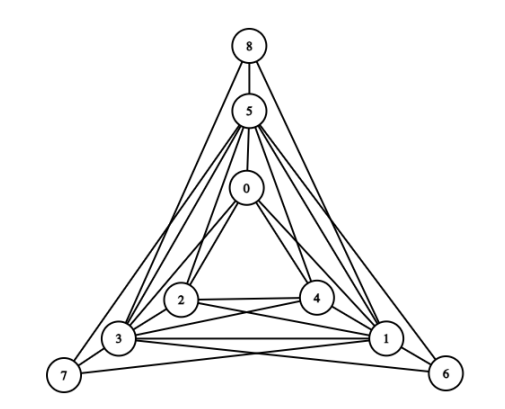
\includegraphics[scale = 0.1]{hw.png}
\end{figure}

We find that for S = \{1, 3, 5\}, c(G-S) = 5 > |S| = 3. Thus G is not Hamiltonian.

problem2:

Graph G is simple. Prove that $\chi(G) + \chi(\overline{G}) \leq n(G) + 1$. Hint: induct on n(G).

sol:Prove by induction on $n(G)$. For $n(G) = 1$, the statement holds because $\chi(G) = \chi(G) = 1$.

Suppose that $n(G) = k > 1$. Consider an arbitrary vertex $v \in V(G)$. We have $|N_G(v)| + |N_{\overline{G}}(v)| = k - 1$. By inductive hypothesis, $\chi(G - v) + \chi(\overline{G - v}) \leq k$.

\textbf{Case 1:} If $\chi(G - v) + \chi(\overline{G - v}) = k > k - 1$, then either $\chi(G - v) > |N_G(v)|$ or $\chi(\overline{G - v}) > |N_{\overline{G}}(v)|$. This is because otherwise we have $\chi(G - v) \leq |N_G(v)|$ and $\chi(\overline{G - v}) \leq |N_{\overline{G}}(v)|$, implying $\chi(G - v) + \chi(\overline{G - v}) \leq |N_G(v)| + |N_{\overline{G}}(v)| = k - 1$, a contradiction. Without loss of generality assume that $\chi(G - v) > |N_G(v)|$. We can then extend an optimal coloring $f'$ of $G - v$ to an optimal coloring $f$ of $G$ by coloring $v$ with some color in $[\chi(G - v)]$ not used by any neighbor of $v$ in $G$, which exists because $\chi(G - v) > |N_G(v)|$. Thus $\chi(G) = \chi(G - v)$, and $\chi(G) + \chi(\overline{G}) \leq \chi(G - v) + \chi(\overline{G - v}) + 1 \leq k + 1$.

\textbf{Case 2:} If $\chi(G - v) + \chi(\overline{G - v}) < k$, then we extend an optimal coloring of $G - v$ to a coloring of $G$ by coloring $v$ with a new color, and extend an optimal coloring of $\overline{G - v}$ to a coloring of $\overline{G}$ by coloring $v$ with a new color. Thus $\chi(G) + \chi(\overline{G}) \leq 1 + 1 + k - 1 = k + 1$.

\end{hw}

% \subsection{hw1}
%     \begin{problem}
%  Prove that no bipartite graph contains an odd cycle    
%     \end{problem}
    
%     \begin{solution}
%     Suppose that A, B-bigraph G contains an odd cycle C = (v1, v2, . . . , v 2k+1). Without loss of generality suppose that v1 $\in$ A. Since G is bipartite and v1 v2 $\in$ E(G), v2 $\in$ B. Similarly, v2 v3 $\in$ E(G)
% and thus v3 $\in$ A, and so on. So v2k+1 $\in$ A. However v1 v2k+1 $\in$ E(G) and yet v1, v 2k+1 $\in$ A, a
% contradiction to the hypothesis that G is an A, B-bigraph.

%     \end{solution}
    
% \subsection{hw2}
%     \begin{problem}
%         Given a simple graph G, $\bar{G}$ is the simple graph with vertex set V(G) such that for any distinct
%  vertices u,v $\in$ V (G), u,v are adjacent in $\bar{G}$ if and only if u,v are not adjacent in G.
%  Prove that at least one of G and $\bar{G}$ is connected.
%     \end{problem}

%     \begin{solution}
%         If G is connected then we are done, so suppose that G is disconnected and has multiple components.
% We aim to prove that any pair of vertices x, y are connected in $\bar{G}$. If x, y belong to different
% components in G, then xy $\notin$ E(G) and xy $\in$ E($\bar{G}$). If x, y belong to the same component C in G,
% then fix a vertex v in a different component in G. Both x, y are adjacent to v in $\bar{G}$, thus x, y are
% connected in $\bar{G}$.

%     \end{solution}

% \subsection{hw3}

% \subsection{hw4}

% \subsection{hw5}

% \subsection{hw6}

\end{CJK*}
\end{document}
